\section{Results}
\label{s:results}
%Results; this should be a readable summary of the results from applying the approach. Don’t pursue death by figures but carefully select what visualisations (figures, tables) are functional for telling your story and logically lead to the main conclusions and policy advice?

% Convincing story, consistent with approach using carefully designed visuals and tables to support narrative
In this section, we summarise the key results from applying this approach, first identifying the most robust policies for Gorssel, Deventer and Overijssel, and subsequently discussing options for synthesising policy choices between the three actors. 


\subsection{Uncertainty Analysis}
Uncertainty Analysis revealed uncertainties in these ranges: x-y

The scenarios selected were based on understanding both how the policies perform under these uncertainty ranges, as well as under a diverse set of 'better' conditions. As such, the two 'worst case' scenarios fall within this uncertainty range, while the remaining scenarios fall across other ranges.

%Z going ham

Before sensitivity analysis and scenario discovery, we found that there is a high correlation between deaths and damages for all actors: $0.09$ for Gorssel, $0.98$ for Deventer, and $0.98$ for Overijssel. Hence, during the remainder of this section, we only target damage.

For the sensitivity analysis on scenarios without any policies, extra trees was employed. It showed that for Gorssel only the durability of their own dike was by far the most dominant (estimator instance of 0.55). For Deventer this dominance was shared by the durability of their own dike and Gorssel's dike (estimator instances of 0.5 and 0.6 respectively). For Overijssel the sensitivity analysis showed the durability of Deventer's dike would be the most dominant (estimator instance of 0.5).

The Prim-algorithm allowed us to zoomed in on certain outcomes. We specifically looked at the worst 10 percentile of damages, and the best 40. Whenever a density $\rho$ with $\rho>0.8$ was reached, we looked at the range of uncertainties. This showed that the durability of Gorssel's dike is also dominant for Overijssel (even though it had an estimator instance of 0.06 during the sensitivity analysis).

What we found odd 

Based on these values the scenarios for the optimisation were selected. In Figure~\ref{fig:prim} we show the values for the selected scenarios for the most dominant sensitive input variables.


\begin{figure}[h]
    \centering
    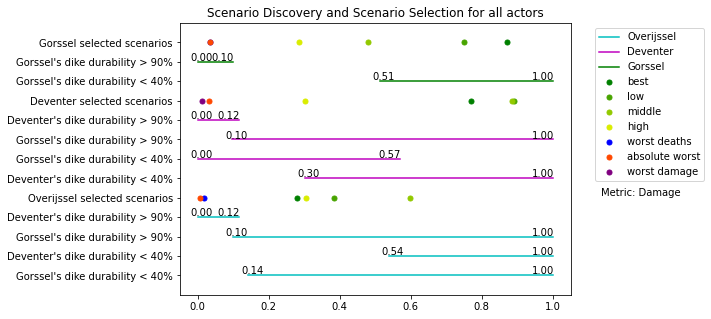
\includegraphics[width=\textwidth]{report/figures/results/scenario_discovery.png}
    \caption{The results from scenario discovery process and the selected scenarios.}
    \label{fig:prim}
\end{figure}


\subsection{Robust Decision Making}
%Look at the policies for the five different scenarios, and examine trade-offs using different robustness metrics.
For the robust decision making process two metrics were used: Satisficing (or the domain-criterion) and maximum regret. 
%#################################################################
%   REGRET AND SATISFICING - GORSSEL
%#################################################################
\subsubsection{Gorssel}
The results from this analysis: The results for Gorssels satisficing analysis with the domain criterion are shown in \autoref{fig:domain_criterion_gorssel}. The 12 selected policies are analysed for trade-offs and how satisficing their results are. \newline
\autoref{fig:domain_criterion_gorssel} shows that every policy is satisficing for "Gorssel Expected Number of Deaths". This means that later policy recommendations, can be sure that the legal standards for citizen safety will be met in "all" scenarios. \newline

Gorssels 'scenario absolute worst option 2' performs best for the domain-criterion results. The policy reaches the highest domain-criterion scores on average. However this policy comes with a big trade-off with the expected annual damage, where the policy often goes over the annual damage budget, and thus reaches a low domain-criterion value for 'expected annual damage'. This would make the policy less robust in terms of damage and more in terms of costs. For the other policies it is the other way around. Most policies except for 'scenario absolute worst option 2' score 0 on 'total costs' and these policies are thus not robust, when considering only satisficing results.  

\autoref{fig:regret_gorssel} shows the results for Gorssel's regret analysis. 



\begin{figure}[H]
  \centering
  \begin{minipage}[b]{0.4\textwidth}
    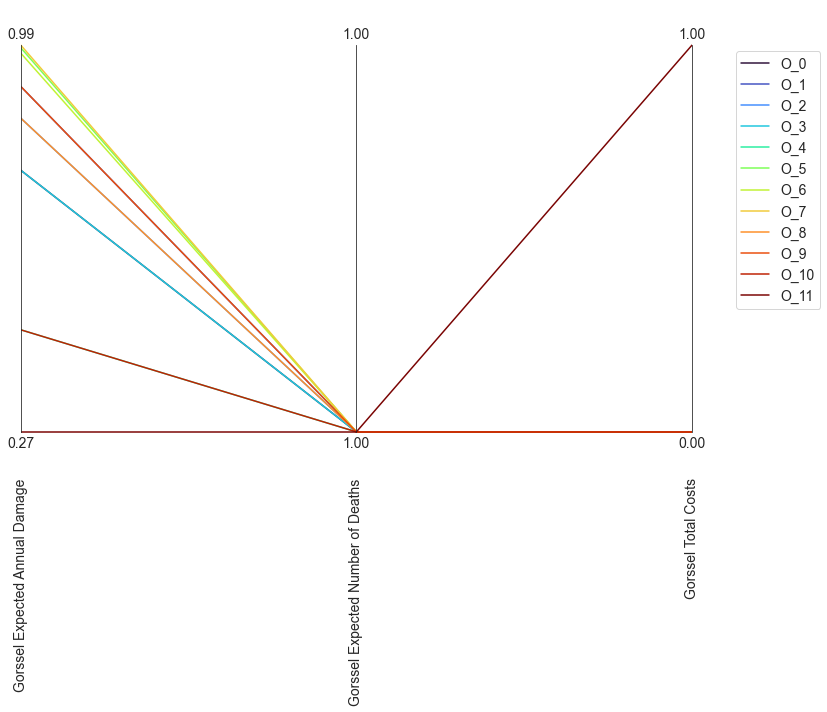
\includegraphics[width=1.15\textwidth]{report/figures/results/domain_criterion_Gorssel.png}
    \caption{Results for Gorssels domain criterion}
    \label{fig:domain_criterion_gorssel}
  \end{minipage}
  \hfill
  \begin{minipage}[b]{0.4\textwidth}
    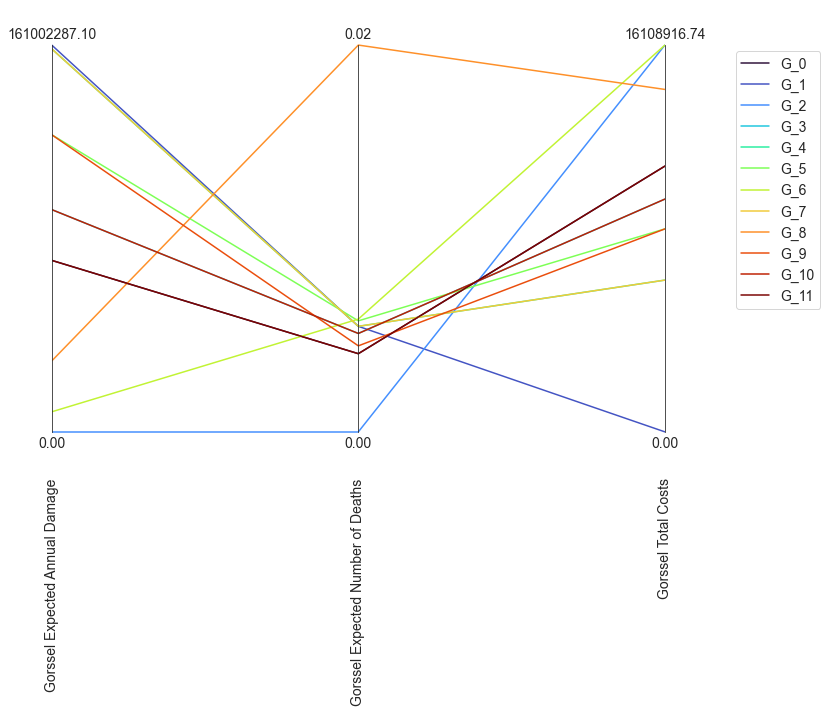
\includegraphics[width=1.15\textwidth]{report/figures/results/regret_figure_Gorssel.png}
    \caption{Results for Gorssel's maximum regret}
    \label{fig:regret_gorssel}
  \end{minipage}
\end{figure}




%#################################################################
%   REGRET AND SATISFICING - DEVENTER
%#################################################################
\subsubsection{Deventer}

\begin{figure}[H]
  \centering
  \begin{minipage}[b]{0.4\textwidth}
    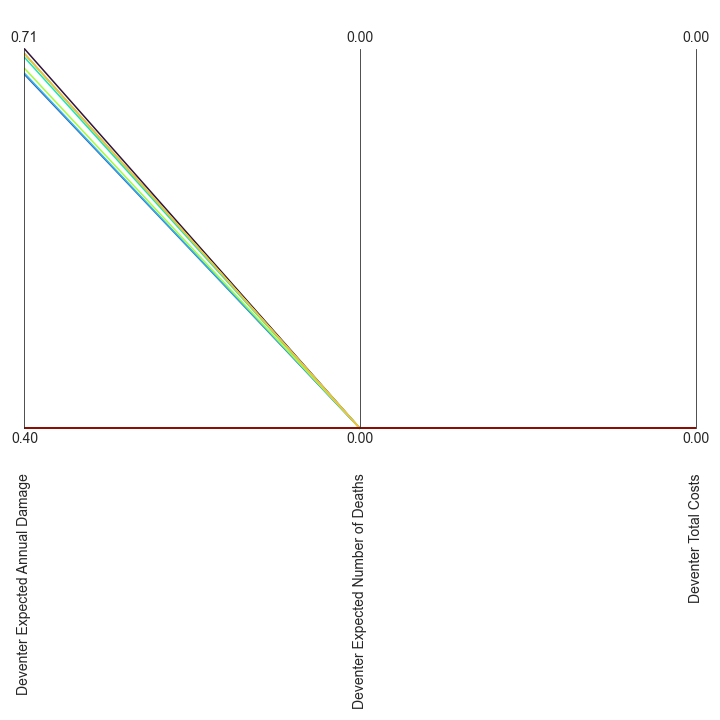
\includegraphics[width=1.15\textwidth]{report/figures/results/domain_criterion_Deventer.png}
    \caption{Results for Deventer's domain criterion}
    \label{fig:domain_criterion_Deventers}
  \end{minipage}
  \hfill
  \begin{minipage}[b]{0.4\textwidth}
    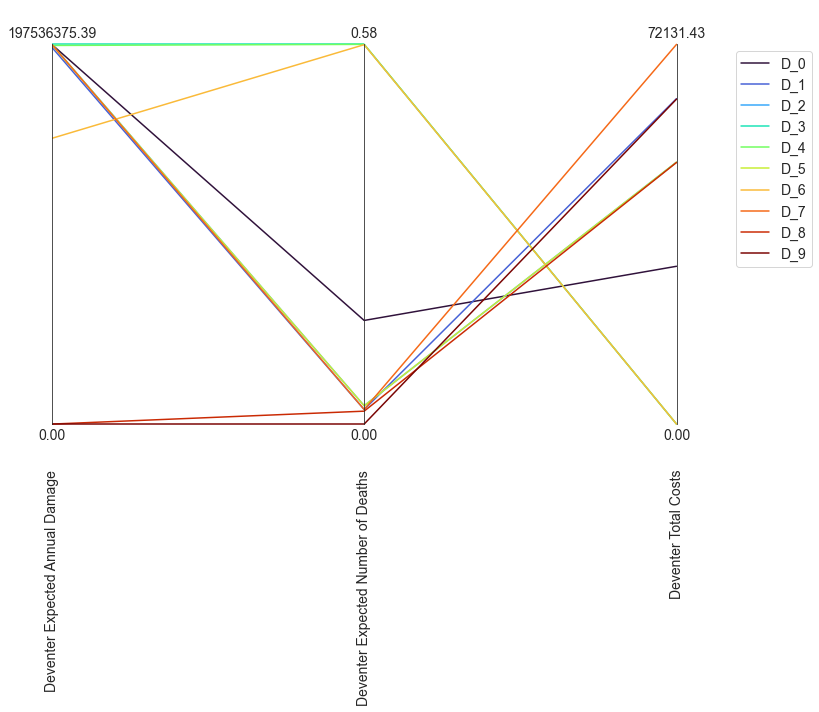
\includegraphics[width=1.15\textwidth]{report/figures/results/regret_figure_Deventer.png}
    \caption{Results for Deventer's maximum regret}
    \label{fig:regret_Deventers}
  \end{minipage}
\end{figure}

%#################################################################
%   REGRET AND SATISFICING - OVERIJSSEL
%#################################################################
\subsubsection{Overijssel}

\begin{figure}[H]
  \centering
  \begin{minipage}[b]{0.4\textwidth}
    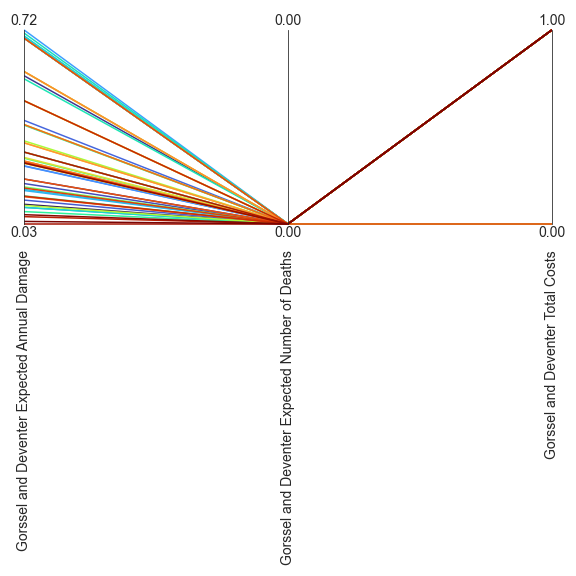
\includegraphics[width=1.15\textwidth]{report/figures/results/domain_criterion_Overijssel.png}
    \caption{Results for Overijssel's domain criterion}
    \label{fig:domain_criterion_Overijssels}
  \end{minipage}
  \hfill
  \begin{minipage}[b]{0.4\textwidth}
    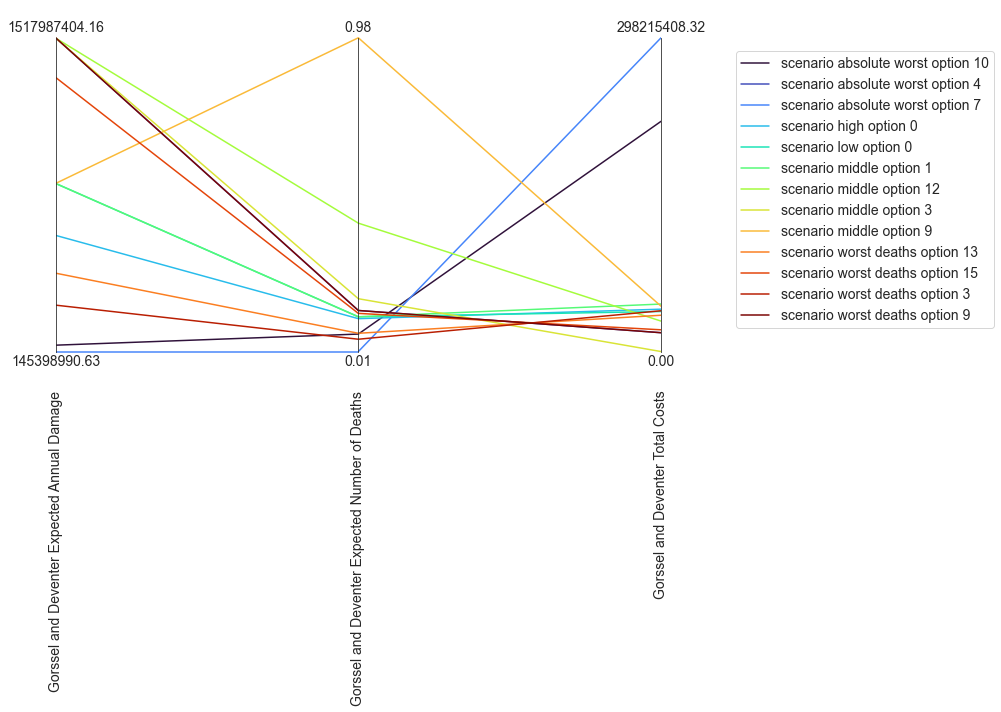
\includegraphics[width=1.15\textwidth]{report/figures/results/regret_figure_Overijssel.png}
    \caption{Results for Overijssel's maximum regret}
    \label{fig:regret_Overijssels}
  \end{minipage}
\end{figure}

\subsection{Shortlisted policies for each Actor}
From the robustness analysis, a subset of the top five most robust policies (prioritising regret-based metrics) were identified. Here, a brief description of each policy, and the relevant actions in terms of dike heightening, room the the river projects, and early warning systems are presented for each actor. The damage, death, and cost outcomes are not included in these tables, as they are already assumed to have been optimised to be within acceptable levels based on the robustness metrics in previous steps.
\subsubsection{Gorssel}
The five most robust policies for Gorssel are presented in Table \ref{fig:gpols}

\begin{figure}[h]
    \centering
    \caption{Robust policies for Gorssel. RfR stands for Room for the River, dike increases are in decimetres and aggregated over all planning steps, EWS refers to Early Warning System in days}
    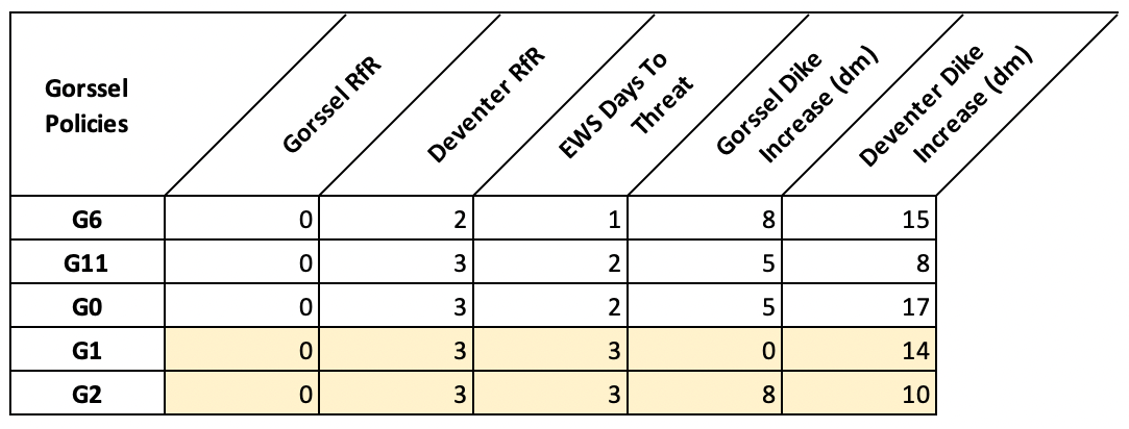
\includegraphics[width=0.4\textwidth]{report/figures/gpols.png}
    \label{fig:gpols}
\end{figure}




\subsubsection{Deventer}
The five most robust policies for Deventer are presented in Table \ref{fig:dpols}

\begin{figure}[h]
    \centering
    \caption{Robust policies for Deventer. RfR stands for Room for the River, dike increases are in decimetres and aggregated over all planning steps, EWS refers to Early Warning System in days}
    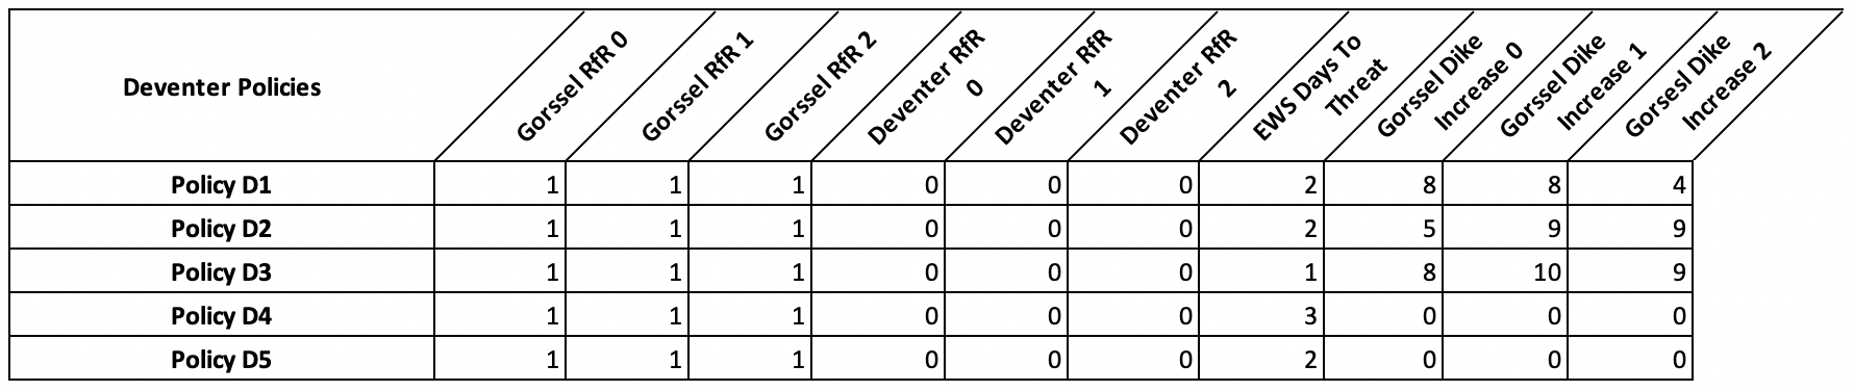
\includegraphics[width=0.4\textwidth]{report/figures/dpols.png}
    \label{fig:dpols}
\end{figure}

\subsubsection{Overijssel}
The five most robust policies for Overijssel are presented in Table \ref{fig:opols}

\begin{figure}[h]
    \centering
    \caption{Robust policies for Overijssel. RfR stands for Room for the River, dike increases are in decimetres and aggregated over all planning steps, EWS refers to Early Warning System}
    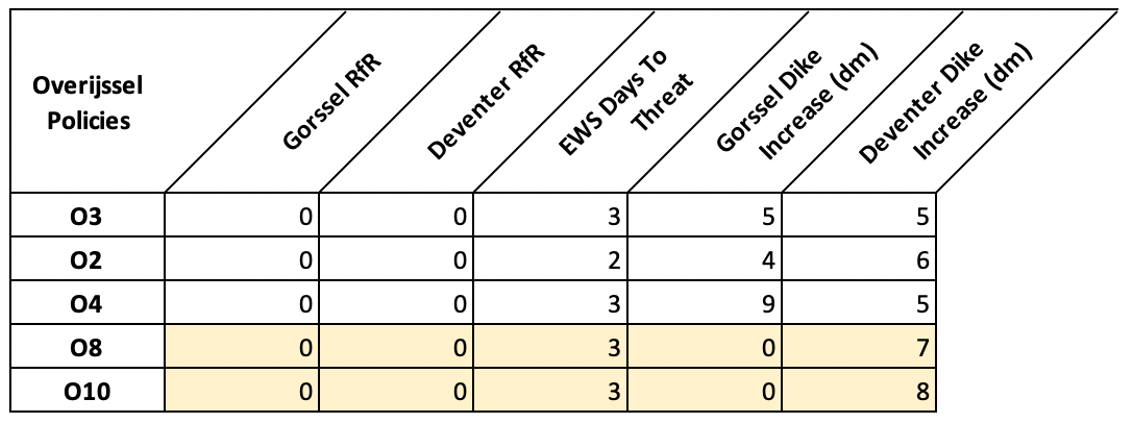
\includegraphics[width=0.4\textwidth]{report/figures/opols.png}
    \label{fig:opols}
\end{figure}

Overijssel's policies prioritise dike increases in the first planning step, with none of the policies prioritising Room for the River (reflecting the relative expense of these policies compared to dike increases). Of interest to Gorssel is policies O8 and O10 (highlighted yellow in the table). These two policies are favourable for both Gorssel and Overijssel (given minimal investment costs in Gorssel), and present an opportunity for starting discussions with Overijssel Province for pursuing such a policy.


\subsection{Sensitivity Analysis}

To see which policies and uncertainties have a large effect on model behaviour, a sensitivity analysis is carried out. The analysis of these can be viewed per actor in the following section. Firstly, the sensitivity analysis was done with feature scoring without the policies to get a grasp of which uncertainty the actors would be most sensitive to. After, policies are added and analysed to assess whether they would be sensitive or not. The generated figures for the sensitivity analysis can be found in Appendix \ref{a:sensitivity-analysis}/

\subsubsection{Gorssel}

From the sensitivity analysis for damage and deaths for Gorssel it becomes apparent that they are not only influenced by their own dike failure, but also by that of Deventer. This has to do with the fairness criteria specified by Gorssel, where they strive to achieve fairness between all actors in the Overijssel province. As a result, the failures of \textit{both} cities have the highest impact on the deaths and damage. When adding the policies, we observe that the sensitivity to dike failure remains the highest for both the deaths and damage. 

\subsubsection{Deventer}

For Deventer the biggest threat to damages and deaths is the dike failure of just Deventer. This is in line with expectations, because only their own dikes breaking would impact Deventer. And just as with Gorssel, we can observe that when adding the policies, we see that the outcome is still least robust under dike failure. 

\subsubsection{Overijssel}

For the costs of the province of Overijssel it can be observed that they are sensitive to dike increase. The sensitivity is biggest to dike increase in Gorssel, which is in line with reality as this is the most costly procedure in the province, other than Room for the River. However, because none of the policies for Overijssel recommend Room for the River, there is no observed sensitivity. Furthermore, the entire province shows a higher score on deaths and damages across the province as well when it comes to dike failure. 

\subsection{Policy Comparison}
Here, the top five policies from each actor are considered and compared to investigate opportunities for coalition forming, or to identify sources of tension in the policy-making process.